\documentclass[12pt,letterpaper]{article}
\usepackage{graphicx,textcomp}
\usepackage{natbib}
\usepackage{setspace}
\usepackage[margin=1in]{geometry}
\usepackage{color}
\usepackage[reqno]{amsmath}
\usepackage{amsthm}
\usepackage{fancyvrb}
\usepackage{amssymb,enumerate}
\usepackage[all]{xy}
\usepackage{endnotes}
\usepackage{lscape}
\newtheorem{com}{Comment}
\usepackage{float}
\usepackage{hyperref}
\newtheorem{lem} {Lemma}
\newtheorem{prop}{Proposition}
\newtheorem{thm}{Theorem}
\newtheorem{defn}{Definition}
\newtheorem{cor}{Corollary}
\newtheorem{obs}{Observation}
\usepackage[compact]{titlesec}
\usepackage{dcolumn}
\usepackage{tikz}
\usetikzlibrary{arrows}
\usepackage{multirow}
\usepackage{xcolor}
\newcolumntype{.}{D{.}{.}{-1}}
\newcolumntype{d}[1]{D{.}{.}{#1}}
\definecolor{light-gray}{gray}{0.65}
\usepackage{url}
\usepackage{listings}
\usepackage{color}

\definecolor{codegreen}{rgb}{0,0.6,0}
\definecolor{codegray}{rgb}{0.5,0.5,0.5}
\definecolor{codepurple}{rgb}{0.58,0,0.82}
\definecolor{backcolour}{rgb}{0.95,0.95,0.92}

\lstdefinestyle{mystyle}{
	backgroundcolor=\color{backcolour},   
	commentstyle=\color{codegreen},
	keywordstyle=\color{magenta},
	numberstyle=\tiny\color{codegray},
	stringstyle=\color{codepurple},
	basicstyle=\footnotesize,
	breakatwhitespace=false,         
	breaklines=true,                 
	captionpos=b,                    
	keepspaces=true,                 
	numbers=left,                    
	numbersep=5pt,                  
	showspaces=false,                
	showstringspaces=false,
	showtabs=false,                  
	tabsize=2
}
\lstset{style=mystyle}
\newcommand{\Sref}[1]{Section~\ref{#1}}
\newtheorem{hyp}{Hypothesis}

\title{Problem Set 2}
\date{Due: October 23, 2025}
\author{Applied Stats/Quant Methods 1}

\begin{document}
	\maketitle
	\section*{Instructions}
\begin{itemize}
	\item Please show your work! You may lose points by simply writing in the answer. If the problem requires you to execute commands in \texttt{R}, please include the code you used to get your answers. Please also include the \texttt{.R} file that contains your code. If you are not sure if work needs to be shown for a particular problem, please ask.
	\item Your homework should be submitted electronically on GitHub.
	\item This problem set is due before 23:59 on Thursday October 23, 2025. No late assignments will be accepted.

\end{itemize}

	
	\vspace{.5cm}
	\section*{Question 1: Political Science}
		\vspace{.25cm}
	The following table was created using the data from a study run in a major Latin American city.\footnote{Fried, Lagunes, and Venkataramani (2010). ``Corruption and Inequality at the Crossroad: A Multimethod Study of Bribery and Discrimination in Latin America. \textit{Latin American Research Review}. 45 (1): 76-97.} As part of the experimental treatment in the study, one employee of the research team was chosen to make illegal left turns across traffic to draw the attention of the police officers on shift. Two employee drivers were upper class, two were lower class drivers, and the identity of the driver was randomly assigned per encounter. The researchers were interested in whether officers were more or less likely to solicit a bribe from drivers depending on their class (officers use phrases like, ``We can solve this the easy way'' to draw a bribe). The table below shows the resulting data.

\newpage
\begin{table}[h!]
	\centering
	\begin{tabular}{l | c c c }
		& Not Stopped & Bribe requested & Stopped/given warning \\
		\\[-1.8ex] 
		\hline \\[-1.8ex]
		Upper class & 14 & 6 & 7 \\
		Lower class & 7 & 7 & 1 \\
		\hline
	\end{tabular}
\end{table}

\begin{enumerate}
	
	\item [(a)]
	Calculate the $\chi^2$ test statistic by hand/manually (even better if you can do "by hand" in \texttt{R}).\\ [0.3cm]
\underline{\textbf{Step 1:} assumptions} 
\begin{itemize}
	\item categorical variables: class and police behaviour (whether they stopped the drivers and requested a bribe from them)
	\item the observations are independent 
	\item the frequency in all cells is above 5 - does not fully apply in this case, but we will proceed anyway (as mentioned in the second footnote)
\end{itemize}
\underline{\textbf{Step 2:} hypotheses} 
\begin{itemize}
	\item null hypothesis: the variables (class and police behaviour) are statistically independent. 
	\item alternative hypothesis: the variables (class and police behaviour) are statistically dependent. 
\end{itemize}
\underline{\textbf{Step 3:} calculate the test statistic} 
\begin{itemize}
	\item set up the data and create a contingency table 
\lstinputlisting[language=R, firstline=22, lastline=31]{PS02_DP.R}
\begin{verbatim}
            Not stopped Bribe requested Stopped/given warning Sum
Upper Class          14               6                     7  27
Lower Class           7               7                     1  15
Sum                  21              13                     8  42
\end{verbatim}
	\item extract the grand total from the contingency table
	\item calculate the expected frequencies using the formula : \\ expected frequency = row total * column total / grand total 
\lstinputlisting[language=R, firstline=34, lastline= 44]{PS02_DP.R}
	\item create a matrix containing the expected frequencies 
\lstinputlisting[language=R, firstline=47, lastline= 53]{PS02_DP.R}
\begin{verbatim}
            Not stopped Bribe requested Stopped/given warning
Upper Class        13.5        8.357143              5.142857
Lower Class         7.5        4.642857              2.857143
\end{verbatim}
	\item having both the observed and the expected frequencies, we can calculate the chi-square test statistic : 
\lstinputlisting[language=R, firstline=56, lastline= 57]{PS02_DP.R}
\begin{verbatim}
	[1] 3.791168
\end{verbatim}
\end{itemize}
	\vspace{0.5cm}
	
	\item [(b)]
	Now calculate the p-value from the test statistic you just created (in \texttt{R}).\footnote{Remember frequency should be $>$ 5 for all cells, but let's calculate the p-value here anyway.}  What do you conclude if $\alpha = 0.1$?\\ [0.3cm]
\underline{\textbf{Step 4:} calculate the p-value} 
\lstinputlisting[language=R, firstline=59, lastline= 65]{PS02_DP.R}
\begin{verbatim}
	[1] 0.1502306
\end{verbatim}
\underline{\textbf{Step 5:} conclusion} \\ [0.5cm]
The p-value is higher than the alpha value (0.1). Thus, we cannot reject the null hypothesis that the variables (class and police behaviour) are statistically independent. \\ [0.3cm]
	\item [(c)] Calculate the standardized residuals for each cell and put them in the table below.
	\vspace{1cm}
	
	\begin{table}[h]
		\centering
		\begin{tabular}{l | c c c }
			& Not Stopped & Bribe requested & Stopped/given warning \\
			\\[-1.8ex] 
			\hline \\[-1.8ex]
			Upper class  &0.3220306   &-1.641957  &1.523026 \\
			Lower class  &-0.3220306  &1.641957   &-1.523026  \\
		\end{tabular}
	\end{table}
	\lstinputlisting[language=R, firstline=70, lastline= 72]{PS02_DP.R}
	\begin{verbatim}
	            Not stopped Bribe requested Stopped/given warning
	Upper Class   0.3220306       -1.641957              1.523026
	Lower Class  -0.3220306        1.641957             -1.523026
	\end{verbatim}
	\item [(d)] How might the standardized residuals help you interpret the results?  \\ [0.5cm]
	Since none of the standardised residuals’ absolute values are greater than 2, we can infer that the observed frequencies don’t deviate substantially from the expected ones. Additionally, these values of the standardised residuals suggest that we are not likely to reject the null hypothesis that the variables are statistically independent. This also aligns with the result of the chi-square test conducted above. 
\end{enumerate}
\newpage

\section*{Question 2: Economics}
Chattopadhyay and Duflo were interested in whether women promote different policies than men.\footnote{Chattopadhyay and Duflo. (2004). ``Women as Policy Makers: Evidence from a Randomized Policy Experiment in India. \textit{Econometrica}. 72 (5), 1409-1443.} Answering this question with observational data is pretty difficult due to potential confounding problems (e.g. the districts that choose female politicians are likely to systematically differ in other aspects too). Hence, they exploit a randomized policy experiment in India, where since the mid-1990s, $\frac{1}{3}$ of village council heads have been randomly reserved for women. A subset of the data from West Bengal can be found at the following link: \url{https://raw.githubusercontent.com/kosukeimai/qss/master/PREDICTION/women.csv}\\

\noindent Each observation in the data set represents a village and there are two villages associated with one GP (i.e. a level of government is called "GP"). Figure~\ref{fig:women_desc} below shows the names and descriptions of the variables in the dataset. The authors hypothesize that female politicians are more likely to support policies female voters want. Researchers found that more women complain about the quality of drinking water than men. You need to estimate the effect of the reservation policy on the number of new or repaired drinking water facilities in the villages.
\vspace{.5cm}
\begin{figure}[h!]
	\caption{\footnotesize{Names and description of variables from Chattopadhyay and Duflo (2004).}}
	\vspace{.5cm}
	\centering
	\label{fig:women_desc}
	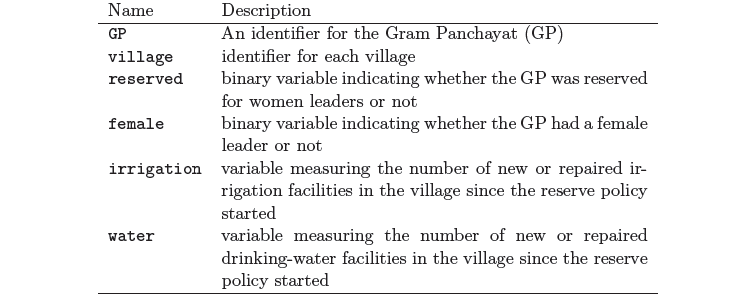
\includegraphics[width=1.1\textwidth]{women_desc.png}
\end{figure}		

\newpage
\begin{enumerate}
	\item [(a)] State a null and alternative (two-tailed) hypothesis. \\ [0.5 cm]
	\textbf{Null hypothesis:} $\beta = 0$ \\
	The reservation policy is not (linearly) associated with the number of new/repaired drinking water facilities in the villages. \\ [0.3cm]
	\textbf{Alternative hypothesis:} $\beta \neq 0$ \\
	The reservation policy is (linearly) associated with the number of new/repaired drinking water facilities in the villages. \\ [0.3cm]
	With $\beta$ being the slope - the coefficient estimate for the reservation policy. 
	
	\vspace{0.5cm}
	\item [(b)] Run a bivariate regression to test this hypothesis in \texttt{R} (include your code!).
\lstinputlisting[language=R, firstline=76, lastline= 82]{PS02_DP.R}
\begin{verbatim}
	Call:
	lm(formula = df$water ~ df$reserved)
	
	Residuals:
	Min      1Q  Median      3Q     Max 
	-23.991 -14.738  -7.865   2.262 316.009 
	
	Coefficients:
	Estimate Std. Error t value Pr(>|t|)    
	(Intercept)   14.738      2.286   6.446 4.22e-10 ***
	df$reserved    9.252      3.948   2.344   0.0197 *  
	---
	Signif. codes:  0 ‘***’ 0.001 ‘**’ 0.01 ‘*’ 0.05 ‘.’ 0.1 ‘ ’ 1
	
	Residual standard error: 33.45 on 320 degrees of freedom
	Multiple R-squared:  0.01688,	Adjusted R-squared:  0.0138 
	F-statistic: 5.493 on 1 and 320 DF,  p-value: 0.0197
\end{verbatim}
	\vspace{6cm}
	\item [(c)] Interpret the coefficient estimate for reservation policy. 
\begin{verbatim}
	Coefficients:
	Estimate Std. Error t value Pr(>|t|)    
	(Intercept)   14.738      2.286   6.446 4.22e-10 ***
	df$reserved    9.252      3.948   2.344   0.0197 *  
\end{verbatim}
	Since the reserved variable is a binary one, the value of the intercept (14.738) shows the average number of new/repaired drinking-water facilities in the villages without the reservation policy. The slope or the coefficient estimate for the reservation policy indicates that, on average, villages where the policy was implemented have 9.252 more new/repaired drinking-water facilities. The p-value (0.0197) is smaller than the signficance level $\alpha=0.05$, so we can reject the null hypothesis that the reservation policy is not associated with the number of new/repaired drinking-water facilities. 
\end{enumerate}
%\end{enumerate}
\end{document}
